\chapter{Learning Relation Classification from the Crowd}
\label{chap:od-rel-ex}

\begin{chapquote}{Ludwig Wittgenstein, \textsc{Tractatus Logico-Philosophicus}}
It is not humanly possible to gather immediately from it what the logic of language is. Language disguises thought.
\end{chapquote}

% \textbf{RQ3:} \textit{Can we improve the performance of natural language processing models by using disagreement-aware ground truth data?}

In this chapter, we investigate whether disagreement-preserving crowdsourcing data can be used to improve the performance of natural language processing models, focusing on the use case of relation extraction from sentences. Distant supervision (DS) is a well-established method for relation extraction from text, based on the assumption that when a knowledge-base contains a relation between a term pair, then sentences that contain that pair are likely to express the relation. We use the results of a crowdsourcing relation extraction task to identify two problems with DS data quality: the widely varying degree of false positives across different relations, and the observed causal connection between relations that are not considered by the DS method. The crowdsourcing data aggregation is performed using ambiguity-aware CrowdTruth metrics, that are used to capture and interpret inter-annotator disagreement. We also explore the problem of propagating human annotation signals gathered for open-domain relation classification through the CrowdTruth methodology for crowdsourcing. We present preliminary results of using the crowd to enhance DS training data for a relation classification model, without requiring the crowd to annotate the entire set. Finally, we present a method that propagates crowd annotations to sentences that are similar in a low dimensional embedding space, expanding the number of labels by two orders of magnitude. Our experiments show significant improvement in a sentence-level multi-class relation classifier.

This chapter is based on the following publications:

\begin{itemize}

\item \textit{False Positive and Cross-relation Signals in Distant Supervision Data} in the Automated Knowledge Base Construction Workshop at NeurIPS 2017, co-authored by Lora Aroyo and Chris Welty~\cite{dumitrache2017false};

\item \textit{Crowdsourcing Semantic Label Propagation in Relation Classification} in the Fact Extraction and Verification Workshop at EMNLP 2018, co-authored by Lora Aroyo and Chris Welty~\cite{dumitrache2018crowdsourcing}.

\end{itemize}

\section{Introduction}

Distant supervision (DS)~\cite{mintz2009distant,Welty:2010:LSR} is a well-established semi-supervised method for performing relation extraction from text. It is based on the assumption that, when a knowledge-base contains a relation between a pair of terms, then any sentence that contains that pair is likely to express the relation. This approach can generate false positives, as not every mention of a term pair in a sentence means a relation is also expressed~\cite{DBLP:conf/ijcai/FengGQLL17}. Furthermore, dependencies between the semantics of the relations such as causality or contradiction are also not considered by the DS methodology. It is often assumed that these disadvantages are compensated for by the scale of the data a DS method can produce, or can be largely overcome with crowdsourced human annotation~\cite{angeli2014combining,liu2016effective}.  

In this chapter, we investigate the question on whether \textit{disagreement-preserving crowdsourcing data can be used to improve the performance of a relation classification model}. To achieve this, we present two experiments in correcting DS data with crowdsourcing. In the first experiment, we identify two specific problems we have found with distant supervision training data: the widely varying degree of false positives across different TAC-KBP relation types, and the observed causal connection between relations. We expose these problems using the CrowdTruth~\cite{aroyo2014threesides,aroyo2015truth,aroyo2013crowd} approach to gathering human annotated data, analyze them, and offer preliminary heuristic and statistical approaches to incorporating them back into DS-based training, that provides better sentence-level relation classification results. %, without requiring crowdsourcing on the full set of data.

The second experiment explores the possibility of automatically expanding smaller human-annotated datasets to DS scale using semantic label propagation. \citet{sterckx2016knowledge} first proposed this method to correct labels of sentence dependency paths by using expert annotators, and then propagating the corrected labels to a corpus of DS sentences by calculating the similarity between the labeled and unlabeled sentences in the embedding space of their dependency paths. We adapt and simplify semantic label propagation to propagate labels without computing dependency paths, and using the crowd instead of experts, which is more scalable. Our simplified algorithm propagates crowdsourced annotations from a small sample of sentences to a large DS corpus. To evaluate our approach, we perform an experiment in open domain relation classification in the English-language, using a corpus of sentences~\cite{crowdODrelexdata2016} whose labels have been collected using the CrowdTruth method.


\section{Related Work}

In recent years, researchers have explored unsupervised methods for correcting DS data. For the task of knowledge base completion, \cite{DBLP:conf/ijcai/FengGQLL17} applied memory networks both to correct false positives in the data, and to capture dependencies between relations. For the same task, \cite{Jiang2016RelationEW} developed a loss function that works with multi-label data, in order to capture co-occurring relations. For relation classification from sentences, \cite{DBLP:conf/acl/SantosXZ15} learn embeddings that capture cross-signals between relations. However, these approaches are dependent on training data that can express relation semantics with at least some accuracy. The initial experiments presented in this chapter show the error rate in the DS data can be so high that unsupervised learning becomes unreliable when it comes to capturing cross-relation signals.

Crowdsourcing is a well-used approach to correcting the mistakes in DS by scaling out cheap human annotation. \citet{angeli2014combining} present an active learning approach to select the most useful sentences that need human re-labeling using a query by committee. \citet{zhang2012big} show that labeled data has a statistically significant, but relatively low impact on improving the quality of DS training data, while increasing the size of the DS corpus has a more significant impact. In contrast, ~\citet{liu2016effective} prove that a corpus of labeled sentences from a pool of highly qualified workers can significantly improve DS quality. All of these methods employ large annotated corpora of 10,000 to 20,000 sentences. In our experiment, we show that a comparatively smaller corpus of 2,050 sentences is enough to correct DS errors through semantic label propagation. \citet{levy2017zero} have shown that a small crowdsourced dataset of questions about relations can be exploited to perform zero-shot learning for relation extraction. \citet{pershina2014infusion} use a small dataset of hand-labeled data to generate relation-specific guidelines that are used as additional features in the relation extraction.

We have been studying the problem of collecting human annotations from the crowd using the CrowdTruth methodology \cite{aroyo2013crowd}.  Our method differs in that it gathers many annotations for the same examples, to better reflect properties like ambiguity, human error and spam, and the target semantics \cite{aroyo2014threesides}. As discussed in Chapter~\ref{chap:med-rel-ex}, we have used this method successfully to improve DS results for the task of medical relation extraction, achieving annotation quality equivalent to that provided by medical experts, at less than half the cost.

The label propagation method was introduced by \citet{xiaojin2002learning}, while \citet{Chen:2006:REU:1220175.1220192} first applied it to correct DS, by calculating similarity between labeled and unlabeled examples an extensive list of features, including part-of-speech tags and target entity types. In contrast, our approach calculates similarity between examples in the word2vec~\cite{mikolov2013distributed} feature space, which it then uses to correct the labels of training sentences. This makes it easy to reuse by the state-of-the-art in both relation classification and relation extraction -- convolutional~\cite{ji2017distant} and recurrent neural network methods~\cite{zhou2016attention} that do not use extensive feature sets. To evaluate our approach, we used a simple convolutional neural network to perform relation classification in sentences~\cite{nguyen2015relation}.


\section{Experimental Setup}

\subsection{Data and Crowdsourcing Setup}

For the \textit{relation-based correction experiment}, we asked the crowd annotate 2,500 sentences from the NIST TAC-KBP 2013 English Slotfilling data that were annotated with DS. For the \textit{semantic label propagation experiment}, we augmented this dataset by another 2,050 sentences picked at random from the corpus of~\citet{angeli2014combining}. For both datasets, we collected annotations for 16 popular relations from the open domain that occur between terms of types $Person$, $Organization$ and $Location$, as shown in in Figure~\ref{fig:template},\footnote{The $alternate\ names$ relation appears twice in the list, once referring to alternate names of persons, and the other referring to organizations.}. The resulting corpus also contains candidate term pairs and DS seed relations for each sentence. As some relations are more general than others, the relation frequency in the corpus is slightly unequal -- e.g. $places\ of\ residence$ is more likely to be in a sentence when $place\ of\ birth$ and $place\ of\ death$ occur, but not the opposite.

\begin{figure}[htb!]
\centering
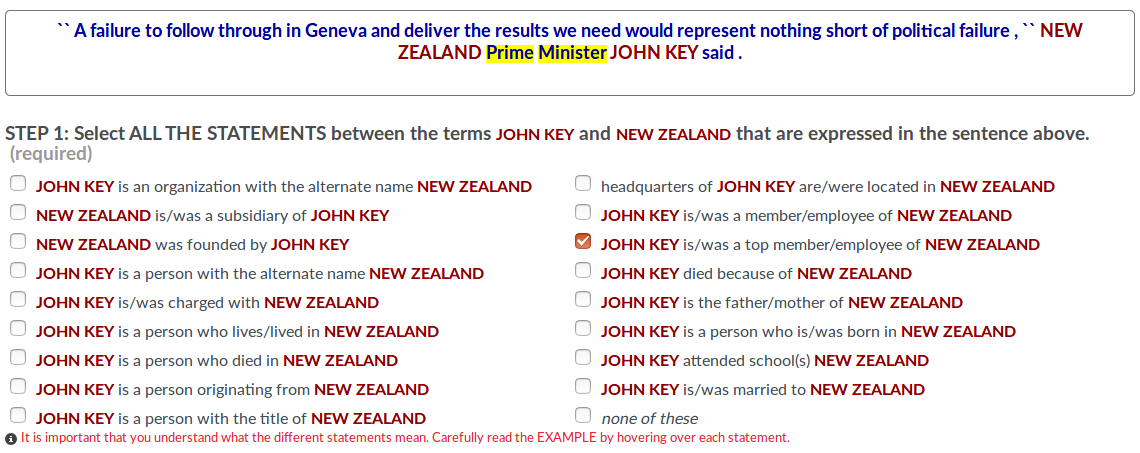
\includegraphics[width=\textwidth]{img/odrelex.png}
\caption{Fragment of the crowdsourcing task template.}
\label{fig:template}
\end{figure}

We ran a multiple-choice crowdsourcing task (Figure~\ref{fig:template}), asking {\em 15 workers to annotate each sentence} with the appropriate relations, or choose the option $none$ if none of the relations presented apply. Workers were encouraged to select all relations that apply. Each worker was paid \$0.05 per sentence. The task was run on the Figure Eight\footnote{\url{https://www.figure-eight.com/}} and Amazon Mechanical Turk\footnote{\url{https://www.mturk.com/}} crowdsourcing platforms. The data is available online~\cite{crowdODrelexdata2016}.


\subsection{CrowdTruth Metrics}

Crowdsourcing annotations are aggregated usually by measuring the consensus of the workers (e.g. using majority vote). This is based on the assumption that a single right annotation exists for each example. In the problem of relation classification, the notion of a single truth is reflected in the fact that a majority of proposed solutions treat relations as mutually exclusive, and the objective of the classification task is usually to find the best relation for a given sentence and term pair. In contrast, the CrowdTruth methodology proposes that crowd annotations are inherently diverse~\cite{aroyo2015truth}, due to a variety of factors such as the ambiguity that is inherent in natural language. We use a comparatively large number of workers per sentences (15) in order to collect inter-annotator disagreement, which results in a more fine-grained ground truth that separates between clear and ambiguous expressions of relations. This is achieved by labeling examples with the inter-annotator agreement on a continuous scale, as opposed to using binary labels.

To aggregate the results of the crowd, we use CrowdTruth metrics\footnote{\url{https://github.com/CrowdTruth/CrowdTruth-core}}~\cite{dumitrache2018crowdtruth} to capture and interpret inter-annotator disagreement as quality metrics for the workers, sentences, and relations in the corpus. The annotations of one worker over one sentence are encoded as a binary worker vector with 17 components, one for each relation and including $none$. The quality metrics for the workers, sentences and relations, are based on average cosine similarity over the worker vectors --  e.g. the quality of a worker $w$ is given by the average cosine similarity between the worker vector of $w$ and the vectors of all other workers that annotated the same sentences. These metrics are mutually dependent (e.g. the sentence quality is weighted by the relation quality and worker quality), the intuition being that low quality workers should not count as much in determining sentence quality, and ambiguous sentences should have less of an impact in determining worker quality, etc. Among the CrowdTruth measures discussed in this chapter, we calculate the per-relation \textit{false positive (FP) rate}, the \textit{causal power} between relation pairs (RCP), and the \textit{sentence-relation score}. Spam removal was performed as well, but the details of this process are not relevant for the chapter.

For each sentence-relation pair, we compute the \textit{sentence-relation score ($srs$)} as the ratio of workers that picked that relation over the total of number of workers, weighted by the worker and relation quality. The $srs$ measures how clearly the relation is expressed in the sentence (the higher the score, the more likely the relation is expressed), and is used as a continuous truth measure. In order to make our results compatible with discrete evaluation metrics (e.g. P, R, F1), we have chosen a threshold of 0.5 per relation, corresponding to the majority vote, that allows for multiple relations to be considered correct in a sentence.  False positive rates are then computed per relation using this threshold.

\textit{Causal power}~\cite{cheng1997causalpower} is an estimate of the probability that the presence of one relation implies the presence of another. Given two relations $i$ and $j$, $ RCP(R_i, R_j) = [ P(R_{j} | R_{i} ) - P(R_{j} | \neg R_{i} ) ] / [1 - P(R_{j} | \neg R_{i} )]$, where $P(R_{i})$ is the probability that relation $R_i$ is annotated in the sentence. This probability can be calculated on a micro basis giving us the probability of one worker annotating two relations together; the \textit{macro RCP} calculates the probabilities in the sentence vectors, capturing causality as a result of two relations being annotated together in the same sentence, but not necessarily by the same workers.  We found micro RCP to be vastly inferior to macro RCP, which is further evidence of the value of having multiple workers per sentence, and only include the macro RCP results in this chapter.


\subsection{Label Propagation}

Inspired by the semantic label propagation method~\cite{sterckx2016knowledge}, we propagate the vectors of $srs$ scores on each crowd annotated sentence to a much larger set of distant supervised (DS) sentences (see datasets description in Section~\ref{sec:train}), scaling the vectors linearly by the distance in low dimensional word2vec vector space~\cite{mikolov2013distributed}.  One of the reasons we chose the CrowdTruth set for this experiment is that the annotation vectors give us a score \emph{for each relation} to propagate to the DS sentences, which have only one binary label.

 Similarly to~\citet{sultan2015dls}, we calculate the vector representation of a sentence as the average over its word vectors, and like \citet{sterckx2016knowledge} we get the similarity between sentences using cosine similarity. Additionally, we restrict the sentence representation to only contain the words between the term pair, in order to reduce the vector space to the one that is most likely to express the relations. For each sentence $s$ in the DS dataset, we find the sentence $l'$ from the crowd annotated set that is most similar to $s$: $ l' = \argmax\limits_{l \in Crowd} cos\ sim(l, s). $ The score for relation $r$ of sentence $s$ is calculated as the weighted average between the $srs(l', r)$ and the original DS annotation, weighted by the cosine similarity to $s$ ($ cos\ sim(s,s) = 1$ for the DS term, and $ cos\ sim(s, l')$ for the $srs$ term):
\begin{equation} \label{eq:ds_w2v}
DS^{*}(s, r) =  \dfrac{DS(s, r) +  cos\ sim(s, l') \cdot srs(l', r)}{1 +  cos\ sim(s, l')}
\end{equation}
\noindent where $DS(s, r) \in \{0,1\}$ is the original DS annotation for the relation $r$ on sentence $s$.


\subsection{Training the Relation Classification Model}
\label{sec:train}

The relation classification model employed is based on~\citet{nguyen2015relation}, who implement a convolutional neural network with four main layers: an embedding layer for the words in the sentence and the position of the candidate term pair in the sentence, a convolutional layer with a sliding window of variable length of 2 to 5 words that recognizes n-grams, a pooling layer that determines the most relevant features, and a softmax layer to perform classification.

We have adapted this model to be both multi-class and multi-label -- we use a sigmoid cross-entropy loss function instead of softmax cross-entropy, and the final layer is normalized with the sigmoid function instead of softmax -- in order to make it possible for more than one relation to hold between two terms in one sentence. The loss function is computed using continuous labels instead of binary positive/negative labels, in order to accommodate the use of the $srs$ in training. The features of the model are the word2vec embeddings of the words in the sentences, together with the position embeddings of the two terms that express the relation. The word embeddings are initialized with 300-dimensional word2vec vectors pre-trained on the Google News corpus\footnote{\url{https://code.google.com/archive/p/word2vec/}}. Both the position and word embeddings are nonstatic and become optimized during training of the model. The values of the other hyper-parameters are the same as those reported by \citet{nguyen2015relation}. The model was implemented in Tensorflow~\cite{abadi2016tensorflow}, and trained in a distributed manner on the DAS-5 cluster~\cite{bal2016medium}.

% We use this model to perform two experiments: (1) a preliminary experiment with \textit{relation-based correction} of the DS data, that shows the potential of disagreement-aware crowdsourcing to correct DS data at scale, without requiring the crowd to annotate the entire set, and (2) an experiment with \textit{semantic label propagation} that shows a robust way of propagating the information in a small crowdsourced corpus to the scale needed for training relation classification models.


\section{Results and Discussion}

In this section, we discuss the results of our experiments on improving the performance of relation classification models with CrowdTruth. First, we evaluate DS data quality using crowdsourced data as ground truth. Next, we present experimental results for two methods to enhance DS training data for relation classification: (1) a preliminary experiment with \textit{relation-based correction} of the DS data, that shows the potential of disagreement-aware crowdsourcing to correct DS data at scale, without requiring the crowd to annotate the entire set, and (2) an experiment with \textit{semantic label propagation} that shows a robust way of propagating the information in a small crowdsourced corpus to the scale needed for training relation classification models.


\subsection{Evaluating DS with CrowdTruth}
\label{sec:ds-eval}

\begin{figure}[htb!]
\centering
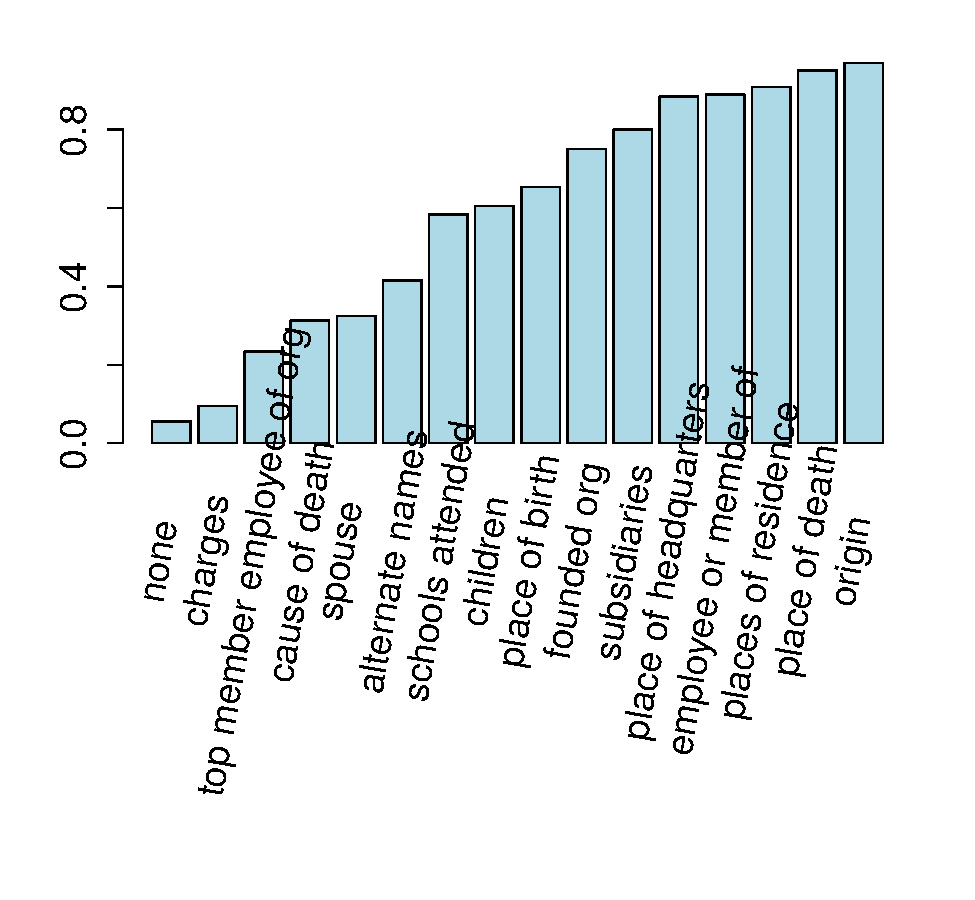
\includegraphics[width=0.65\textwidth]{img/fp_ratio.pdf}
\caption{DS ratio of false positive over all positive labels, using the crowd as ground truth.}
\label{fig:fp_rate}
\end{figure}

Using the $srs$ as a ground truth at a 0.5 threshold, Figure~\ref{fig:fp_rate} shows the correctness of the DS labels on the initial dev set of 1,025 sentence. There is \textit{considerable variation in DS data quality across relations}. The $origin$ and $place\ of\ death$ relations scored particularly badly, with more than 90\% false positives. With such a high error rate in some relations, it is arguable that any classifier could learn anything meaningful, regardless of algorithm or quantity of data.

Manual error analysis on the initial dev set showed that many sentences contain a $Person$ - $Location$ pair, where freebase specified both that the person resided in and died at that location. This makes intuitive sense, people tend to die in the places they live.  In most of these cases, the sentence expressed only the $places\ of\ residence$ relation, leading to the false positives. The $origin$ relation data suffers from the same problem.  Table~\ref{tab:ds_fp_ex} in the Appendix~\ref{sec:appendix4.1} shows several examples of these sentences. This led us to consider a heuristic solution to this problem as a headroom study as well as a statistical solution. Both are discussed in Section 5.

\begin{table}[htb!]
\centering
\begin{subfigure}{\textwidth}
    \centering
    \scalebox{0.8}{
    \begin{tabular}{rccccccc}
    \toprule
          & PoB   & O     & PoR   & PoD   & FO  & EoM     & TEoM \\ \toprule
     PoB  & 1     & \textbf{0.64}  & 0.17  & -0.12 & -0.19 & -0.2  & -0.21  \\ 
     \cellcolor{aliceblue}O    & \cellcolor{aliceblue}\textbf{0.88}  & \cellcolor{aliceblue}1     & \cellcolor{aliceblue}0.31  & \cellcolor{aliceblue}-0.16 & \cellcolor{aliceblue}-0.29 & \cellcolor{aliceblue}-0.22 & \cellcolor{aliceblue}-0.22 \\ 
     PoR  & 0.42  & \textbf{0.56}  & 1     & \textbf{-0.1}  & -0.59 & 0.12  & 0.13 \\ 
     \cellcolor{aliceblue}PoD  & \cellcolor{aliceblue}-0.03 & \cellcolor{aliceblue}-0.03 & \cellcolor{aliceblue}-0.01 & \cellcolor{aliceblue}1     & \cellcolor{aliceblue}-0.04 & \cellcolor{aliceblue}-0.05 & \cellcolor{aliceblue}-0.05 \\ 
     FO   & -0.07 & -0.07 & -0.09 & -0.06 & 1     & 0.1   & 0.13 \\ 
     \cellcolor{aliceblue}EoM  & \cellcolor{aliceblue}-0.45 & \cellcolor{aliceblue}-0.36 & \cellcolor{aliceblue}0.11  & \cellcolor{aliceblue}-0.47 & \cellcolor{aliceblue}0.62  & \cellcolor{aliceblue}1     & \cellcolor{aliceblue}0.82 \\ 
     TEoM & -0.5  & -0.38 & 0.13  & -0.45 & 0.86  & \textbf{0.86}  & 1 \\ %\hline
     \bottomrule
    \end{tabular}
    }
	\caption{Crowd-based RCP}
    \label{tab:crowd_rcp}
\end{subfigure}
\begin{subfigure}{\textwidth}
    \centering
    \scalebox{0.8}{
    \begin{tabular}{rccccccc}
    \toprule
           & PoB   & O     & PoR   & PoD   & FO    & EoM   & TEoM \\ \toprule
     PoB   & 1     & \textbf{-0.6}  & 0.55  & -0.14 & -0.54 & -0.48 & -0.57 \\ 
     \cellcolor{aliceblue}O     & \cellcolor{aliceblue}\textbf{-0.02} & \cellcolor{aliceblue}1     & \cellcolor{aliceblue}-0.11 & \cellcolor{aliceblue}-0.16 & \cellcolor{aliceblue}-0.16 & \cellcolor{aliceblue}0.19  & \cellcolor{aliceblue}-0.15 \\ 
     PoR   & 0.65  & \textbf{-0.33} & 1     & \textbf{0.45}  & -0.7  & -0.68 & -0.75 \\  
     \cellcolor{aliceblue}PoD   & \cellcolor{aliceblue}-0.06 & \cellcolor{aliceblue}-0.18 & \cellcolor{aliceblue}0.17  & \cellcolor{aliceblue}1     & \cellcolor{aliceblue}-0.18 & \cellcolor{aliceblue}-0.13 & \cellcolor{aliceblue}-0.19 \\ 
     FO    & -0.08 & -0.06 & -0.09 & -0.06 & 1     & 0.09  & 0.09 \\ 
     \cellcolor{aliceblue}EoM   & \cellcolor{aliceblue}-0.35 & \cellcolor{aliceblue}0.35  & \cellcolor{aliceblue}-0.42 & \cellcolor{aliceblue}-0.21 & \cellcolor{aliceblue}0.46  & \cellcolor{aliceblue}1     & \cellcolor{aliceblue}0.66 \\ 
     TEoM  & -0.16 & -0.1  & -0.17 & -0.12 & 0.34  & \textbf{0.24}  & 1 \\ \bottomrule
    \end{tabular}
    }
	\caption{DS-based RCP.}
    \label{tab:ds_rcp}
\end{subfigure}
\caption{RCP for relation subset: $place\ of\ birth$ (PoB), $origin$ (O), $places\ of\ residence$ (PoR), $place\ of\ death$ (PoD), $founded\ organization$ (FO), $employee\ or\ member$ (EoM), $top\ employee\ or\ member$ (TEoM). The scores show the causal power $RCP(R_i, R_j)$ of relations $R_i$ in the rows, over the relations $R_j$ in the columns. Significant changes between crowd annotation based causal power and distant supervision are in bold.}
\label{tab:rcp}
\end{table}

The results of the macro RCP analysis for six of the relations we analyzed (Table \ref{tab:rcp}) shows that the $place\ of\ birth$ relation has a high causal power (0.64) over $origin$, meaning that when $place\ of\ birth$ is annotated in a sentence, $origin$ is also likely to appear, with the inverse causal power at 0.88.  This high co-causality seems to indicate a confusion between the two relations. Note also that these two relations have significant differences in causal power in the DS-based data. In contrast, $place\ of\ death$ has a high causal power over $places\ of\ residence$ in the DS data (0.45), reflecting the high error rate of $place\ of\ death$ caused by the overlap in the KB with $places\ of\ residence$.

In the crowd data we see a much higher co-causality for \\ $employee\ or\ member$ and $top\ employee\ or\ member$, with only a slight preference in the data for what we expect to be the ``correct'' causal direction (that $top\ employee\ or\ member$ causes $employee\ or\ member$), but in the DS-based analysis, the incorrect interpretation drops a lot. In manual error analysis we observed that these are properties of the data set, which talk about more famous people who tend to be leaders and founders, not ``regular'' employees.  Table~\ref{tab:ds_fn_ex} in the Appendix shows several examples sentences with false negative DS labels due to missing causality.

Among the non-symmetric causal pairs we see that \\ $top\ employee\ or\ member$ causes $founded\ organization$, $employee\ or\ member$ causes $founded\ org$, and $top\ employee\ or\ member$ causes $founded\ org$.  These again appear to be properties of the data set.


\subsection{Relation-Based Correction Experiment}

We expect that the metrics from CrowdTruth annotation can be used to systematically enhance DS data at scale, without requiring the crowd to annotate the entire set.  As a preliminary headroom exercise, we trained three models to test a few simple heuristic characterizations of our analysis, and compared them to a baseline trained purely on DS data. In each model, we changed only the training set (using the methods described below). Each model was trained for 20,000 iterations, after the point of stabilization for the train loss. We used the data in our initial held-out test set as an evaluation target, again processing the continuous SRS scores with a threshold of 0.5 to yield discrete truth values for calculating P, R, and F. To evaluate the relation classification model on CrowdTruth data with discrete metrics, we set a comparable threshold of 0.5 on the model confidence score, separating between negative and positive labels. Results are shown in Table ~\ref{tab:cnn_res}.

\begin{enumerate}

\item \textbf{DS:} The baseline of 235,000 sentences annotated by DS from freebase relations, used in~\citet{riedel2013relation}. The per-relation training labels are binary ($1$ and $0$), based on the results of DS.

\item \textbf{DS merged:} Based on the results of the causality analysis, the training set is augmented to reflect the highest cross-relation signals.  We merge relations with symmetric RCP ($origin$ and $place\ of\ birth$), and add the implied relation in the case of asymmetric RCP ($employee\ or\ member$  and $top\ employee\ or\ member$). To merge, the \textbf{DS} baseline data is updated so that the symmetric relations always co-occur, and adding caused relation whenever the caused relation appears. This approach shows a huge improvement across the board over the baseline, with the overall highest P and F.

\item \textbf{DS\_RCP:} Instead of manually identifying merged relations, the training data is augmented by using the RCP scores. When a relation $i$ has a positive \textbf{DS} label for a given sentence, the labels of all other relations $j \neq i$ are updated by adding the macro RCP that $i$ has over $j$. The maximum value for the label is clipped at 1, to keep scores in the $[0,1]$ interval. The training labels in this set have continuous values, as opposed to the binary values in the previous two sets. The formula for updating the training label for relation $j$ in sentence $s$ is: $ DS\ RCP(s, j) = max[1, DS(s, j) + \sum_{i \neq j} RCP(i,j) \cdot DS(s,i) ],$ where $DS(s,i)$ is the DS label of relation $i$ in sentence $s$.  This method was comparable in precision to the baseline, but scored a huge win in recall.  The recall increase makes sense, though we have yet to investigate or explain the lack of increase in precision.

\item \textbf{DS\_FP:} Our analysis showed that the $place\ of\ death$ relation was a large source of false positives in the DS data, because most of the positives were actually expressing $places\ of\ residence$.  In every sentence in the DS training set that had a 1 for $place\ of\ death$, we updated the score by subtracting its false positive ratio, which was used in the loss function as described above.  This did not impact the results over the baseline, mainly because there were not many $place\ of\ death$ relations in the DS data nor the test set, and any improvement did not impact the overall result.  We are confident that more systematic treatment of false positive rates will improve performance.

\end{enumerate}

\begin{table}[htb!]
\centering
\scalebox{0.8}{
\begin{tabular}{rccc}
\toprule
& \textsc{Precision} & \textsc{Recall} &\textsc{F1 score} \\ \toprule
\textsc{DS} & 0.19 & 0.22 & 0.2 \\
\textsc{DS merged} & \textbf{0.43} & 0.33 & \textbf{0.37}  \\
\textsc{DS\_RCP} & 0.19 & \textbf{0.48} & 0.27 \\
\textsc{DS\_FP} & 0.21 & 0.22 & 0.21  \\ % \hline
\bottomrule
\end{tabular}
}
\caption{Precision \& Recall at 20,000 training steps.}
\label{tab:cnn_res}
\end{table}

The differences (in bold in Table \ref{tab:rcp}) between the crowd and DS-based causal power accounts for some of the classification errors in our trained system, and we expect them to be a significant cause of error in systems that try to learn cross-relation signals from DS data alone.

The preliminary results are not overwhelming, but highly indicative. There is considerable headroom in cross-relation signals, and a more robust approach holds promise to eliminate manual analysis, and work as part of an overall pipeline that includes partial crowd data.


\subsection{Label Propagation Experiment}

Building on the results from the previous section on, we studied \textit{label propagation} as a more robust method of using a small crowdsourced corpus to augment a DS dataset larger by several orders of magnitude. As opposed to relation-based correction methods, label propagation takes into account the information contained in the sentences themselves, providing a more fine-grained method to correct errors in DS.

For this experiment, we split the full 4,100 crowd sentences into a dev and a test set of equal size, and trained three models to compare with the baseline on the held-out test set. Each model is trained for 25,000 iterations, after the point of stabilization for the train loss. The models were trained by the following datasets:

\begin{enumerate}
\item \textbf{DS:} The baseline of 235,000 sentences annotated by DS.
\item \textbf{DS + CT:} The 2,050 crowd dev annotated sentences added directly to the DS dataset.
\item \textbf{DS + W2V CT:} The DS$^{*}$ dataset (Eq.~\ref{eq:ds_w2v}), with relation scores propagated over the 2,050 crowd dev sentences.
\end{enumerate}

To evaluate the performance of the label propagation method, we calculate the micro precision and recall (Figure~\ref{fig:pr}), as well as the cosine similarity per sentence with the test set (Figure~\ref{fig:cos_sim}).  In order to calculate the precision and recall, a threshold of 0.5 was set in the $srs$, and each sentence-relation pair was labeled either as positive or negative. However, for calculating the cosine similarity, the $srs$ was used without change, in order to better reflect the degree of agreement the crowd had over annotating each example.  We observe that \textbf{DS + W2V CT}, with a precision/recall $AUC = 0.512$, significantly outperforms \textbf{DS} (P/R $AUC = 0.294$). \textbf{DS + CT} (P/R $AUC = 0.372$) also does slightly better than \textbf{DS}, but not enough to compete with the semantic label propagation method. The cosine similarity result (Figure~\ref{fig:cos_sim}) shows that \textbf{DS + W2V CT} also produces model predictions that are closer to the different agreement levels of the crowd. Take advantage of the agreement scores in the CrowdTruth corpus, the cosine similarity evaluation allows us to assess relation confidence scores on a continuous scale. The crowdsourcing results and model predictions are available online~\cite{crowdODrelexdata2016}.

\begin{figure}[tbh!]
\centering
\begin{subfigure}{.5\textwidth}
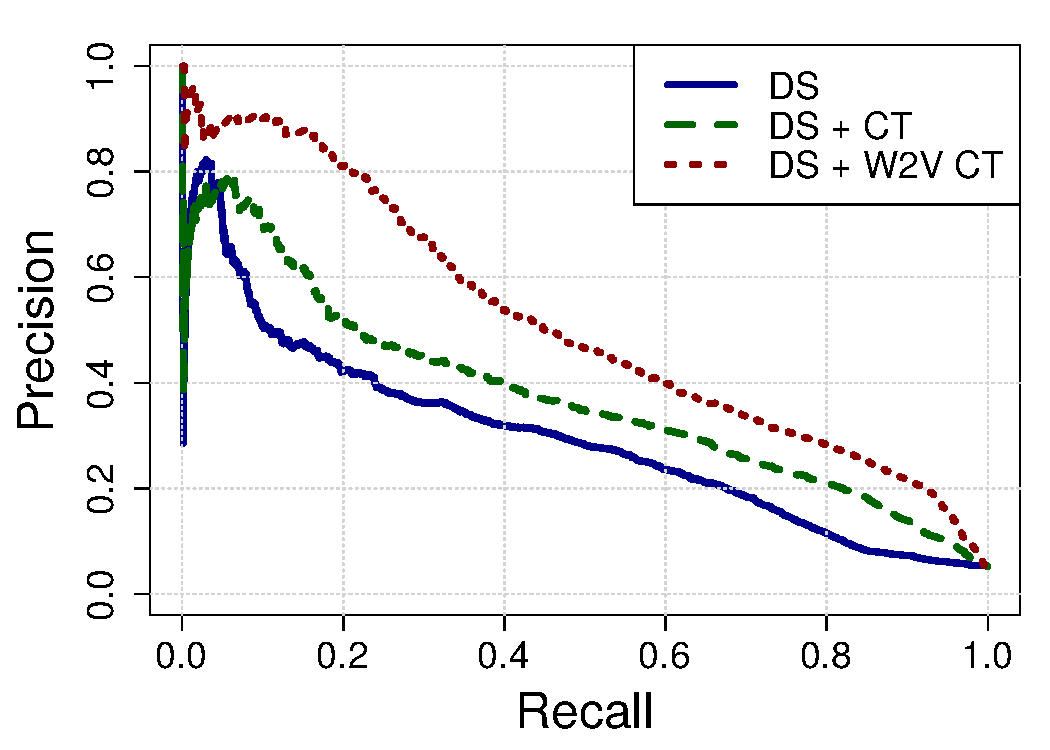
\includegraphics[width=\linewidth]{img/pr.pdf}
\caption{Precision / Recall curve, calculated for each sentence-relation pair.}
\label{fig:pr}
\end{subfigure}%
\begin{subfigure}{.5\textwidth}
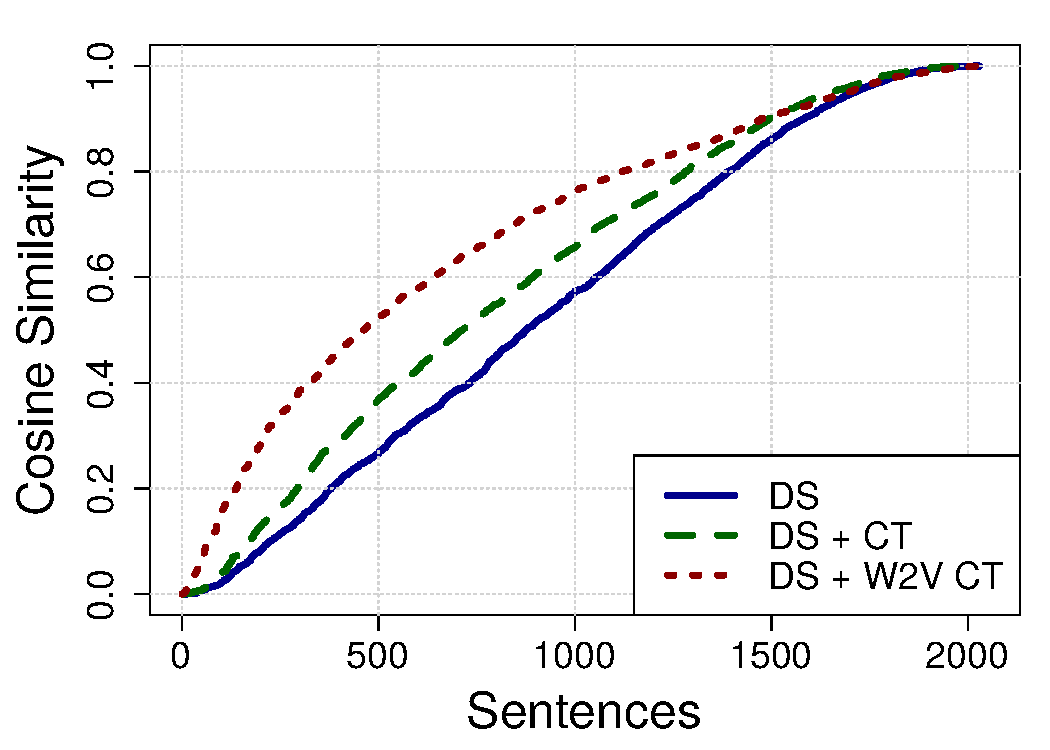
\includegraphics[width=\linewidth]{img/cos_sim.pdf}
\caption{Distribution of sentence-level cosine similarity with test set values.}
\label{fig:cos_sim}
\end{subfigure}
\caption{Label propagation evaluation results.}
\end{figure}

One reason for which the semantic label propagation method works better than simply adding the correctly labeled sentences to the train set is the high rate of incorrectly labeled examples in the DS training data, as discussed in Section~\ref{sec:ds-eval}. %Figure~\ref{fig:fp} shows that some relations, such as $origin$ and $places\ of\ residence$, have a ratio of over 0.8 false positive sentences, meaning that a vast majority of training examples are incorrectly labeled.
The success of the \textbf{DS + W2V CT} comes in part because the method relabels all sentences in DS. Adding correctly labeled sentences to the train set would require a significantly larger corpus in order to correct the high false positive rate, but semantic label propagation only requires a small corpus (two orders of magnitude smaller than the train set) to achieve significant improvements.

% \begin{figure}[hbt!]
% \centering
% 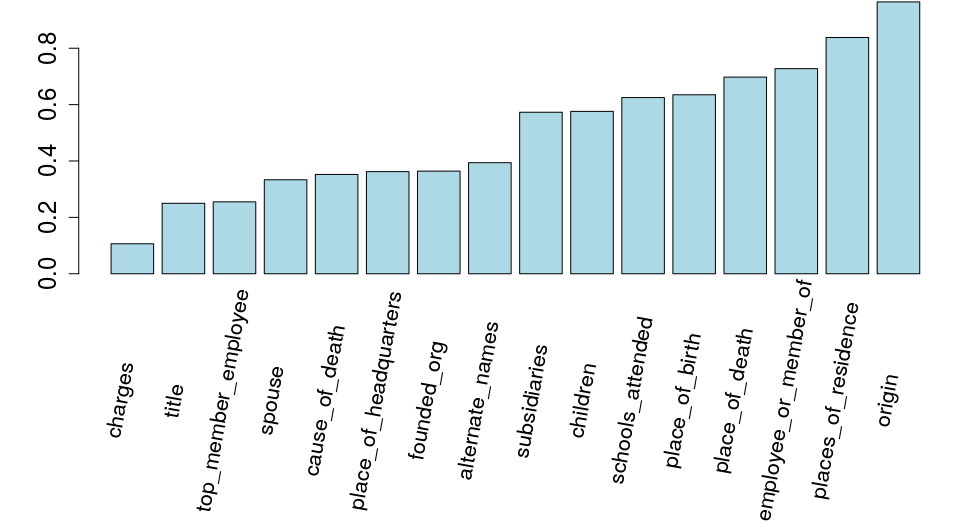
\includegraphics[width=0.75\textwidth]{img/fp.png}
% \caption{DS false positive ratio in combined crowd dev and test sets.}
% \label{fig:fp}
% \end{figure}



\section{Conclusion}

This chapter explores how to \textit{improve the performance of open-domain relation classification models with disagreement-aware ground truth data}, by propagating human annotation signals in distant supervision training data. We have shown a very significant variation in the false positive rate in distant supervision data, and it seems extremely likely that this can be exploited to improve training. We also presented experimental results for two methods to enhance DS training data for relation classification: (1) a preliminary experiment with \textit{relation-based correction} of the DS data, that shows the potential of disagreement-aware crowdsourcing to correct DS data at scale, without requiring the crowd to annotate the entire set, and (2) an experiment with \textit{semantic label propagation} that shows a robust way of propagating the information in a small crowdsourced corpus to the scale needed for training relation classification models.

Our version of the label propagation approach passes on the information in human annotations to sentences that are similar in a low dimensional embedding space, using a small crowdsourced dataset of 2,050 sentences to correct training data labeled with distant supervision.  We present experimental results from training a relation classifier, where our method shows significant improvement over the DS baseline, as well as just adding the labeled examples to the train set. Unlike \citet{sterckx2016knowledge} who employ experts to label the dependency path representation of sentences, our method uses the general crowd to annotate the actual sentence text, and is thus easier to scale and not dependent on methods for extracting dependency paths, so it can be more easily adapted to other languages and domains.  Also, since the semantic label propagation is applied to the data before training is completed, this method can easily be reused to correct train data for any model, regardless of the features used in learning.

In future work, we plan to use the label propagation method to correct training data for state-of-the-art models in relation classification, but also relation extraction and knowledge-base population. We also plan to explore different ways of collecting and aggregating data from the crowd. CrowdTruth~\cite{dumitrache2017false} proposes capturing ambiguity through inter-annotator disagreement, which necessitates multiple annotators per sentence, while \citet{liu2016effective} propose increasing the number of labeled examples added to the training set by using one high quality worker per sentence. We will compare the two methods to determine whether quality or quantity of data are more useful for semantic label propagation. To achieve this, we will investigate whether disagreement-based metrics such as sentence and relation quality can also be propagated through the training data. We believe a more continuous truth measure as opposed to the rather arbitrary discrete measure will be productive for this evaluation. Finally, we are particularly excited about the possibility of using our approach in conjunction with logical reasoning approaches such as those reported in \cite{demeester2016regularizing}.  In this case, we are looking at more informed data that reflects human understanding and properties of the data set, to discover candidate relation pairs for investigating rules. 

\newpage

\section*{Appendix: Example Sentences with Wrong Distant Supervision Labels}
\label{sec:appendix4.1}

\begin{table}[htb!]
\centering
\scalebox{0.8}{
\bgroup
\def\arraystretch{1.5}
\begin{tabular}{p{5cm}c>{\centering\arraybackslash}p{2cm}>{\centering\arraybackslash}p{2cm}}
\toprule
\textsc{Sentence} & \textsc{Relation} & \textsc{Crowd SRS} & \textsc{DS label} \\ \toprule

\multirow{4}{5cm}{After growing up on Cat Island, \textbf{Tony McKay} moved to \textbf{New York City} at age 17 to study architecture.} & \multirow{2}{*}{$place\ of\ death$} & \multirow{2}{*}{0.004} & \multirow{2}{*}{1} \\
& & & \\ %\cline{2-4}
& \multirow{2}{*}{$places\ of\ residence$} & \multirow{2}{*}{0.995} & \multirow{2}{*}{1} \\
& & & \\ \hline

\multirow{4}{5cm}{The film is based very loosely on the lives of \textbf{Wolfgang Amadeus Mozart} and Antonio Salieri, two composers who lived in \textbf{Vienna, Austria}.} & \multirow{2}{*}{$place\ of\ death$} & \multirow{2}{*}{0.074} & \multirow{2}{*}{1} \\
& & & \\ %\cline{2-4}
& \multirow{2}{*}{$places\ of\ residence$} & \multirow{2}{*}{0.865} & \multirow{2}{*}{1} \\
& & & \\ \hline

\multirow{4}{5cm}{Marku Ribas is the side more Black music of this group and was \textbf{Bob Marley}'s friend in the 1970s, \textbf{Jamaica}, where he lived.} & \multirow{2}{*}{$origin$} & \multirow{2}{*}{0} & \multirow{2}{*}{1} \\ 
& & & \\ %\cline{2-4}
& \multirow{2}{*}{$places\ of\ residence$} & \multirow{2}{*}{0.87} & \multirow{2}{*}{1} \\
& & & \\ \hline

\multirow{4}{5cm}{\textbf{Osama bin Laden} had moved from \textbf{Saudi Arabia} to Sudan during the 1990-91 Gulf War.} & \multirow{2}{*}{$origin$} & \multirow{2}{*}{0.3} & \multirow{2}{*}{1} \\
& & & \\ %\cline{2-4}
& \multirow{2}{*}{$places\ of\ residence$} & \multirow{2}{*}{0.74} & \multirow{2}{*}{1} \\
& & & \\ \bottomrule
 
\end{tabular}
\egroup
}
\caption{Example sentences with false positive $place\ of\ death$ and $origin$ DS labels due to multiple relations in the KB over $Person$ - $Location$ term types.}
\label{tab:ds_fp_ex}
\end{table}

\begin{table}[htb!]
\centering
\scalebox{0.8}{
\bgroup
\def\arraystretch{1.5}
\begin{tabular}{p{5cm}c>{\centering\arraybackslash}p{2cm}>{\centering\arraybackslash}p{2cm}}
\toprule
\textsc{Sentence} & \textsc{Relation} & \textsc{Crowd SRS} & \textsc{DS label} \\ \toprule

\multirow{4}{5cm}{China on Monday officially appointed \textbf{Donald Tsang} as \textbf{Hong Kong}'s chief executive for a second term.} & \multirow{2}{*}{$employee\ or\ member$} & \multirow{2}{*}{0.623} & \multirow{2}{*}{0} \\
& & & \\ %\cline{2-4}
& \multirow{2}{*}{$top\ employee\ or\ member$} & \multirow{2}{*}{0.753} & \multirow{2}{*}{1} \\
& & & \\ \hline

\multirow{4}{5cm}{More than 3,000 taxi drivers blocked \textbf{Rome}'s historic centre Wednesday to protest extra licences given by mayor \textbf{Walter Veltroni}.} & \multirow{2}{*}{$employee\ or\ member$} & \multirow{2}{*}{0.529} & \multirow{2}{*}{0} \\
& & & \\ %\cline{2-4}
& \multirow{2}{*}{$top\ employee\ or\ member$} & \multirow{2}{*}{0.841} & \multirow{2}{*}{1} \\
& & & \\ \hline

\multirow{4}{5cm}{Early years \textbf{Joey Harrington} was born and raised in \textbf{Portland, Oregon}, where he has resided his entire life.} & \multirow{2}{*}{$origin$} & \multirow{2}{*}{0.645} & \multirow{2}{*}{0} \\
& & & \\ %\cline{2-4}
& \multirow{2}{*}{$place\ of\ birth$} & \multirow{2}{*}{0.867} & \multirow{2}{*}{1} \\
& & & \\ \hline

\multirow{4}{5cm}{\textbf{Nelli Zhiganshina} (born March 31, 1987 in \textbf{Moscow}, Russia) is a Russian ice dancer who currently represents Germany.} & \multirow{2}{*}{$origin$} & \multirow{2}{*}{0.555} & \multirow{2}{*}{0} \\
& & & \\ %\cline{2-4}
& \multirow{2}{*}{$place\ of\ birth$} & \multirow{2}{*}{0.791} & \multirow{2}{*}{1} \\
& & & \\ %\hline
\bottomrule
 
\end{tabular}
\egroup
}
\caption{Example sentences with false negative $employee\ or\ member$ and $origin$ DS labels due to missing causal connections.}
\label{tab:ds_fn_ex}
\end{table}
